\section{Xamarin.Forms: 3 Native UIs, 1 Shared Code Basis}
Bei Xamarin.Forms handelt es sich um ein .NET-basiertes UI Toolkit, mit dem Oberfl�chen entweder in
C\# oder einem speziellen XAML-Dialekt generisch definiert werden. W�hrend des Kompiliervorgangs
entstehen aus dem gemeinsamen Code plattformspezifische, native Benutzeroberfl�chen. Xamarin.Forms
unterst�tzt die Plattformen iOS, Android und Windows Phone, aber (noch) nicht Windows Store Apps. Mit Xamarin.Forms
k�nnen Entwickler deutlich weniger Code schreiben und dadurch wird der jeweilige Mehraufwand pro zu
unterst�tzende Plattform geringer. Allerdings gibt es (noch) keinen UI Designer bei Xamarin.Forms
und man muss die Benutzeroberfl�chen aus dem Code gestalten.
%%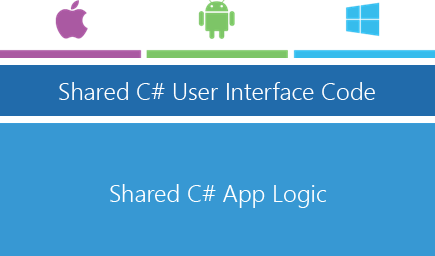
\includegraphics[scale = 0.5]{graphics/XamarinForms1.png}
\\Es gibt zwei
unterschiedliche L�sungsans�tze f�r die plattform�bergreifenden Projekte:
\begin{itemize}
      \item Shared Projects
      \item Portable Class Libraries (PCL)
   \end{itemize}
Bei dem Shared Projects Ansatz wird der enthaltene Code f�r die jeweilige Plattform kopiert und
erneut �bersetzt. Auf diese Weise wird der Code direkt in die Assembly des referenzierenden Projekts
integriert und es wird keine neue Assembly erzeugt. So l�sst sich der Code dieser Assembly auf
mehreren Plattformen wiederverwenden und zugleich �ber Pr�prozessordirektiven oder partielle
Methoden und Klassen in den nativen Projekten auf plattformspezifische Anforderungen eingehen, ohne
zus�tzliche Abstraktionsschichten f�r die nativen Funktionen einbauen zu m�ssen. Allerdings muss
hier erw�hnt werden, dass bei diesem L�sungsansatz die �bersicht im Code schnell verloren geht und
dadurch die Wartbarkeit des Codes erschwert wird. 
\\Bei dem zweiten L�sungsansatz (PCL) bietet sich hingegen die M�glichkeit, mit gemeinsamer
Funktionalit�t ausgew�hlter Zielplattformen gemeinsamen Code in einer Assembly abzubilden. Dadurch
wird ein m�glich effizientes Code Sharing erreicht.
\begin{figure}[!h]
\centering
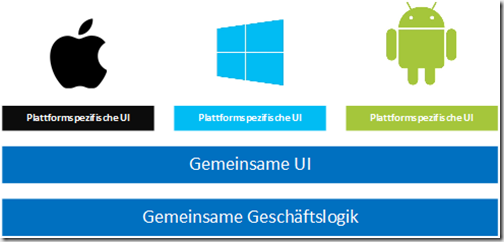
\includegraphics[scale = 0.5]{graphics/xamarin_forms-solution2.png}
\caption{Xamarin.Forms}
\label{fig:abb3}
\end{figure}
\\Die gemeinsame Gesch�ftslogik ist in der
Portable Class Library beinhaltet.
Zus�tzlich werden noch drei weitere Projekte erstellt, eins f�r Android, eins f�r iOS und eins f�r Windows Phone. In den
plattformspezifischen Projekte befinden sich plattformspezifische Views und Logik. Die meisten
Dateien in den plattformspezifischen Projekten werden automatisch generiert. In ganz seltenen F�llen
muss der Entwickler etwas in den plattformspezifischen Projekte hinzuf�gen. Meistens geht es um
Datenbankanbindung oder die Implementierung von Custom Control Renderer, um die von
Xamarin.Forms vorgegebenen Visualisierung von UI Controls zu modifizieren.
%%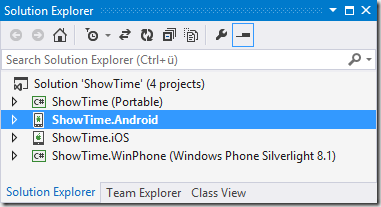
\includegraphics[scale = 0.5]{graphics/xamarin_forms-solution.png}
\\Im Allgemeinen besteht eine Xamarin.Forms Solution aus jeweils einem Projekt pro zu
unterst�tzende Plattform und einem (oder mehreren) plattform�bergreifenden Projekten. 
\begin{figure}[!h]
\centering
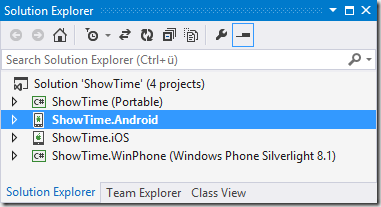
\includegraphics[scale = 0.73]{graphics/xamarin_forms-solution.png}
\caption{Solution}
\label{fig:abb4}
\end{figure}

\section{NuGet und Xamarin Component Store}
Xamarin bietet die M�glichkeit Komponente zu jeder App direkt aus der IDE hinzuzuf�gen.
Somit kann man diverse Controls, Web Service APIs und vieles mehr benutzen. Es k�nnen auch
popul�re Backends wie Microsoft Azure, Parse, Salesforce, SAP usw. in die APP integriert werden,
sowie auch Security Features wie Authentifizierung und Verschl�sselung.

\section{Fazit}
Xamarin.iOS und Xamarin.Android verschaffen direkten Zugriff auf die plattformspezifischen APIs und
dadurch lassen sich Apps erstellen, die spezielle Interaktionen erfordern. Solche Apps haben
die Funktionalit�t und die Leistung einer nativen Anwendung.\\Hingegen ist der Ansatz von
Xamarin.Forms besonders gut f�r Apps geeignet, die wenig plattformspezifische Funktionalit�t
aufweisen oder solche, bei denen keine spezielleren Benutzeroberfl�chen erfordert werden. Also
Anwendungen, bei denen die Gesch�ftslogik h�her priorisiert wird als optische Effekte der
Benutzeroberfl�che, lassen sich ganz bequem mit Xamarin.Forms erstellen. Unter diese Kategorie
fallen die sogenannten Business(Enterprise)-Anwendungen.
